% Shared float (common/make_floats.py). Figure: figures/cnn_ablations.pdf
\begin{figure}[htbp]
\centering
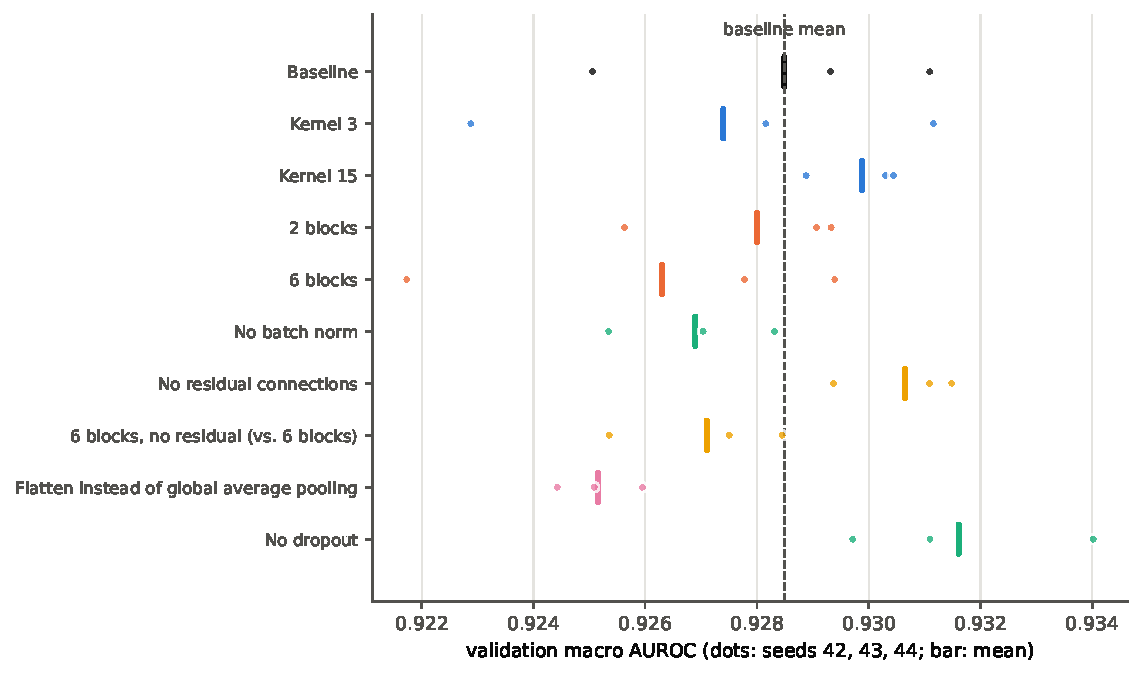
\includegraphics[width=\textwidth,height=0.42\textheight,keepaspectratio]{figures/cnn_ablations.pdf}
\caption[1D CNN: ablations]{CNN ablations: validation macro AUROC of every configuration (dots: seeds 42, 43, 44; bar: mean; dashed line: baseline mean). Note the narrow horizontal range.}
\label{fig:cnn_ablations}
\end{figure}
